


\usepackage[eulerchapternumbers,beramono,pdfspacing]{classicthesis}

%
%\usepackage[
%  eulerchapternumbers,
%  beramono,
%  pdfspacing,
%  hyperref={
%    pdfpagemode=UseOutlines,
%    bookmarks=true,
%    bookmarksopen=true,
%    bookmarksopenlevel=1,
%    bookmarksnumbered=true,
%    hypertexnames=false,
%    colorlinks=true,
%    linkcolor=red,
%    citecolor=green,
%    urlcolor=magenta,
%    filecolor=magenta,
%    pdfstartview=FitV,
%    unicode=true,
%    breaklinks=true
%  }
%]{classicthesis}


\usepackage{arsclassica}







\usepackage{graphicx}

\graphicspath{
  {images/}             
  {../images/}  
}


\usepackage{textcase}
\usepackage{setspace}






%
%\usepackage[
%  eulerchapternumbers,
%  beramono,
%  pdfspacing,
%  hyperref={
%    pdfpagemode=UseOutlines,
%    bookmarks=true,
%    bookmarksopen=true,
%    bookmarksopenlevel=1,
%    bookmarksnumbered=true,
%    hypertexnames=false,
%    colorlinks=true,
%    linkcolor=red,
%    citecolor=green,
%    urlcolor=magenta,
%    filecolor=magenta,
%    pdfstartview=FitV,
%    unicode=true,
%    breaklinks=true
%  }
%]{classicthesis}


%
%%%%%%%%%%%%%%%%%%%%%%%%%%%%%%%%%%%%%%%%%%%%%%%%%%%%%%%%%%%%%%%%%%%%
%%%%%%%%%%%%%%%%%%%%%%%% CHATGPT TITLE PAGE  %%%%%%%%%%%%%%%%%%%%%%%
%%%%%%%%%%%%%%%%%%%%%%%%%%%%%%%%%%%%%%%%%%%%%%%%%%%%%%%%%%%%%%%%%%%%
%\makeatletter
%\renewcommand{\maketitle}{%
%  \begin{titlepage}
%    \begin{center}
%      % --- Title ---
%      {\huge\spacedallcaps{\@title} \par}
%      \vspace{1cm}
%
%      % --- Fun image between title and author ---
%      \includegraphics[width=0.25\textwidth]{images/fun_image.png}\par
%      \vspace{1cm}
%
%      % --- Author ---
%      {\Large \@author \par}
%      \vfill
%
%      % --- Date ---
%      {\large \@date \par}
%    \end{center}
%  \end{titlepage}%
%}
%\makeatother
%
%
%

%
%%%%%%%%%%%%%%%%%%%%%%%%%%%%%%%%%%%%%%%%%%%%%%%%%%%%%%%%%%%%%%%%%%%%
%%%%%%%%%%%%%%%%%%%%%%%% DEEPSEEK TITLE PAGE %%%%%%%%%%%%%%%%%%%%%%%
%%%%%%%%%%%%%%%%%%%%%%%%%%%%%%%%%%%%%%%%%%%%%%%%%%%%%%%%%%%%%%%%%%%%
% Title page customization
%\makeatletter
%\renewcommand{\maketitle}{%
%    \begin{titlepage}
%        \begin{center}
%            \vspace*{1.5cm}
%            
%            % University logo at top
%            
\includegraphics[width=0.3\textwidth]{logo-orizzontale-completo.jpg}\\
%            \vspace{1cm}
%            
%            % Title with decorative rule
%            {\singlespacing\LARGE\spacedlowsmallcaps{\@title}\par}
%            \vspace{0.4cm}
%            \rule{0.5\textwidth}{0.4pt}\par
%            \vspace{1.5cm}
%            
%            % Featured image
%            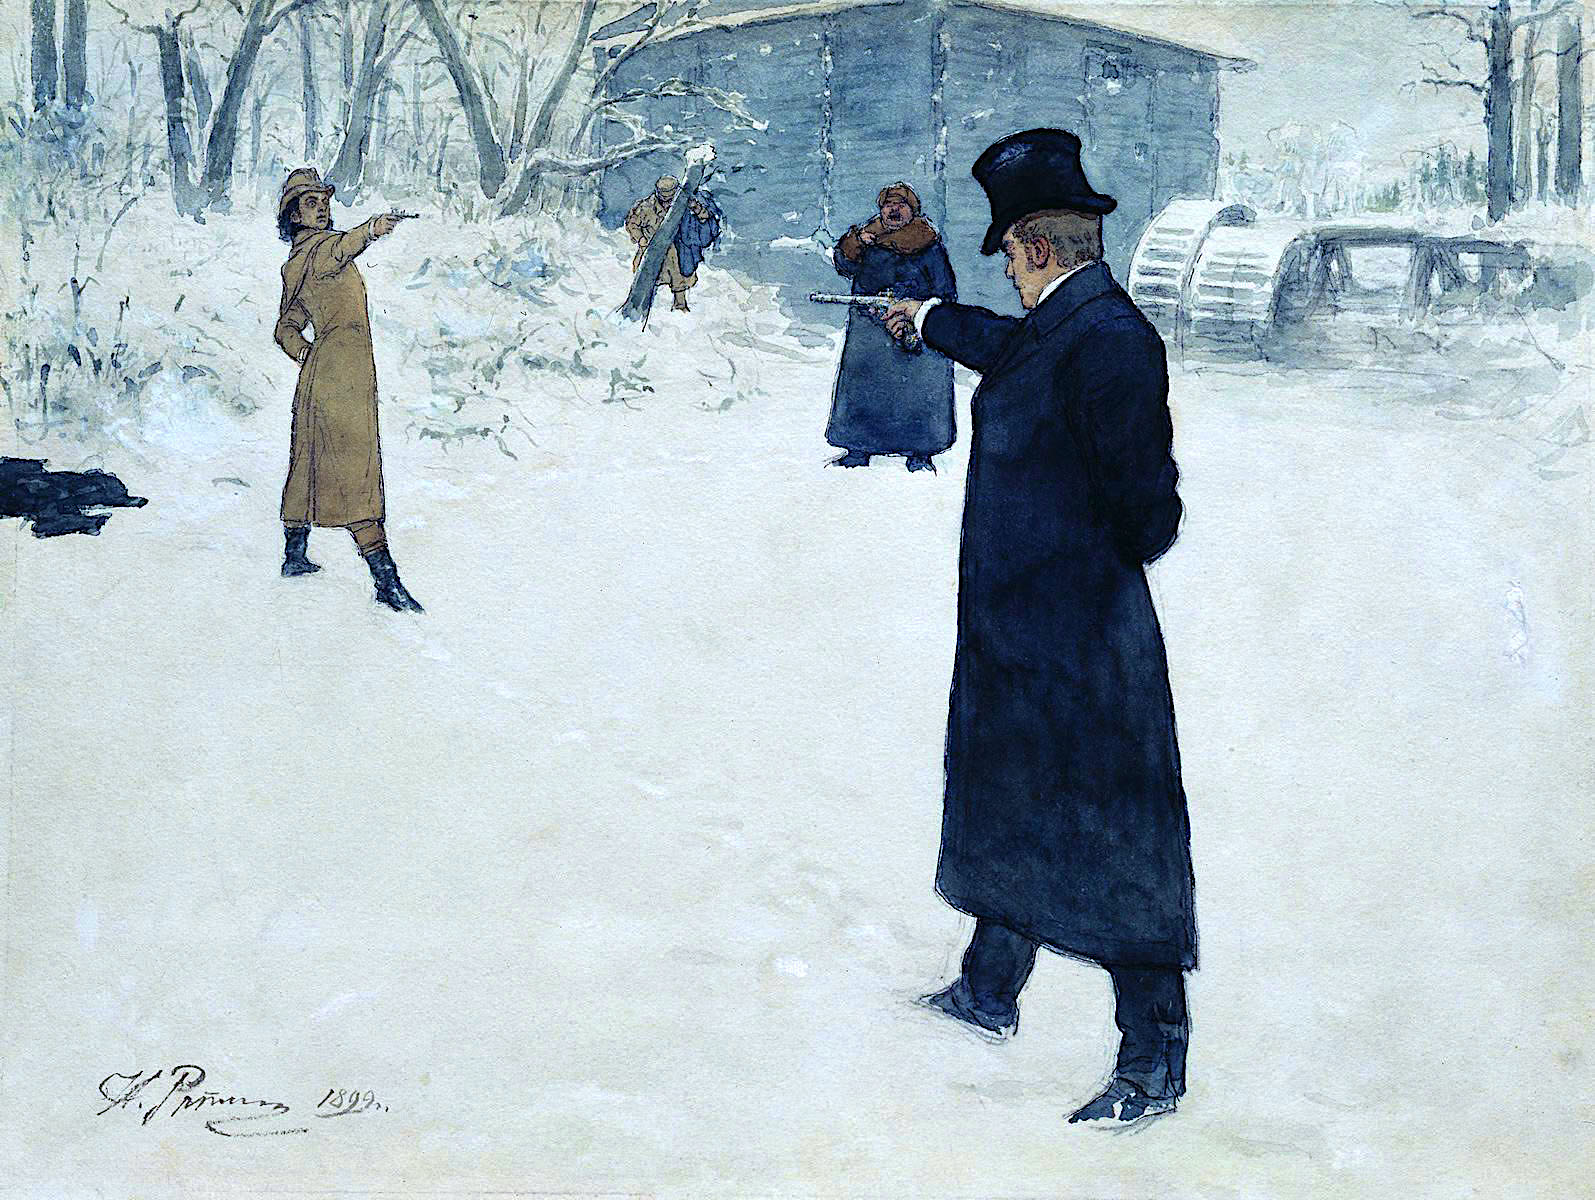
\includegraphics[width=0.9\textwidth]{Eugene}\\
%            \vspace{1.5cm}
%            
%            % Author information
%            {\large\spacedlowsmallcaps{By}\par}
%            \vspace{0.5cm}
%            {\Large\spacedallcaps{\@author}\par}
%            \vspace{1cm}
%            
%            % Department and date
%            {\large Department of Statistics\par}
%            \vspace{0.2cm}
%            {\large University of Data Science\par}
%            \vspace{0.5cm}
%            {\large \@date\par}
%            
%            \vfill
%            
%            % Publisher logo at bottom
%            
\includegraphics[width=0.2\textwidth]{logo-orizzontale-completo.jpg}
%        \end{center}
%    \end{titlepage}
%}
%\makeatother
% Title page customization
\makeatletter
\renewcommand{\maketitle}{%
    \begin{titlepage}
        \begin{center}
            \vspace*{1.5cm}
            
            % University logo at top
     %       
\includegraphics[width=0.3\textwidth]{Logo_HSE.png}\\
            \vspace{1cm}

            % Title with decorative rule
            {\singlespacing\LARGE\spacedlowsmallcaps{\@title}\par}
            \vspace{0.4cm}
            \rule{0.5\textwidth}{0.4pt}\par
            \vspace{1.5cm}

            % Featured image without explanation
            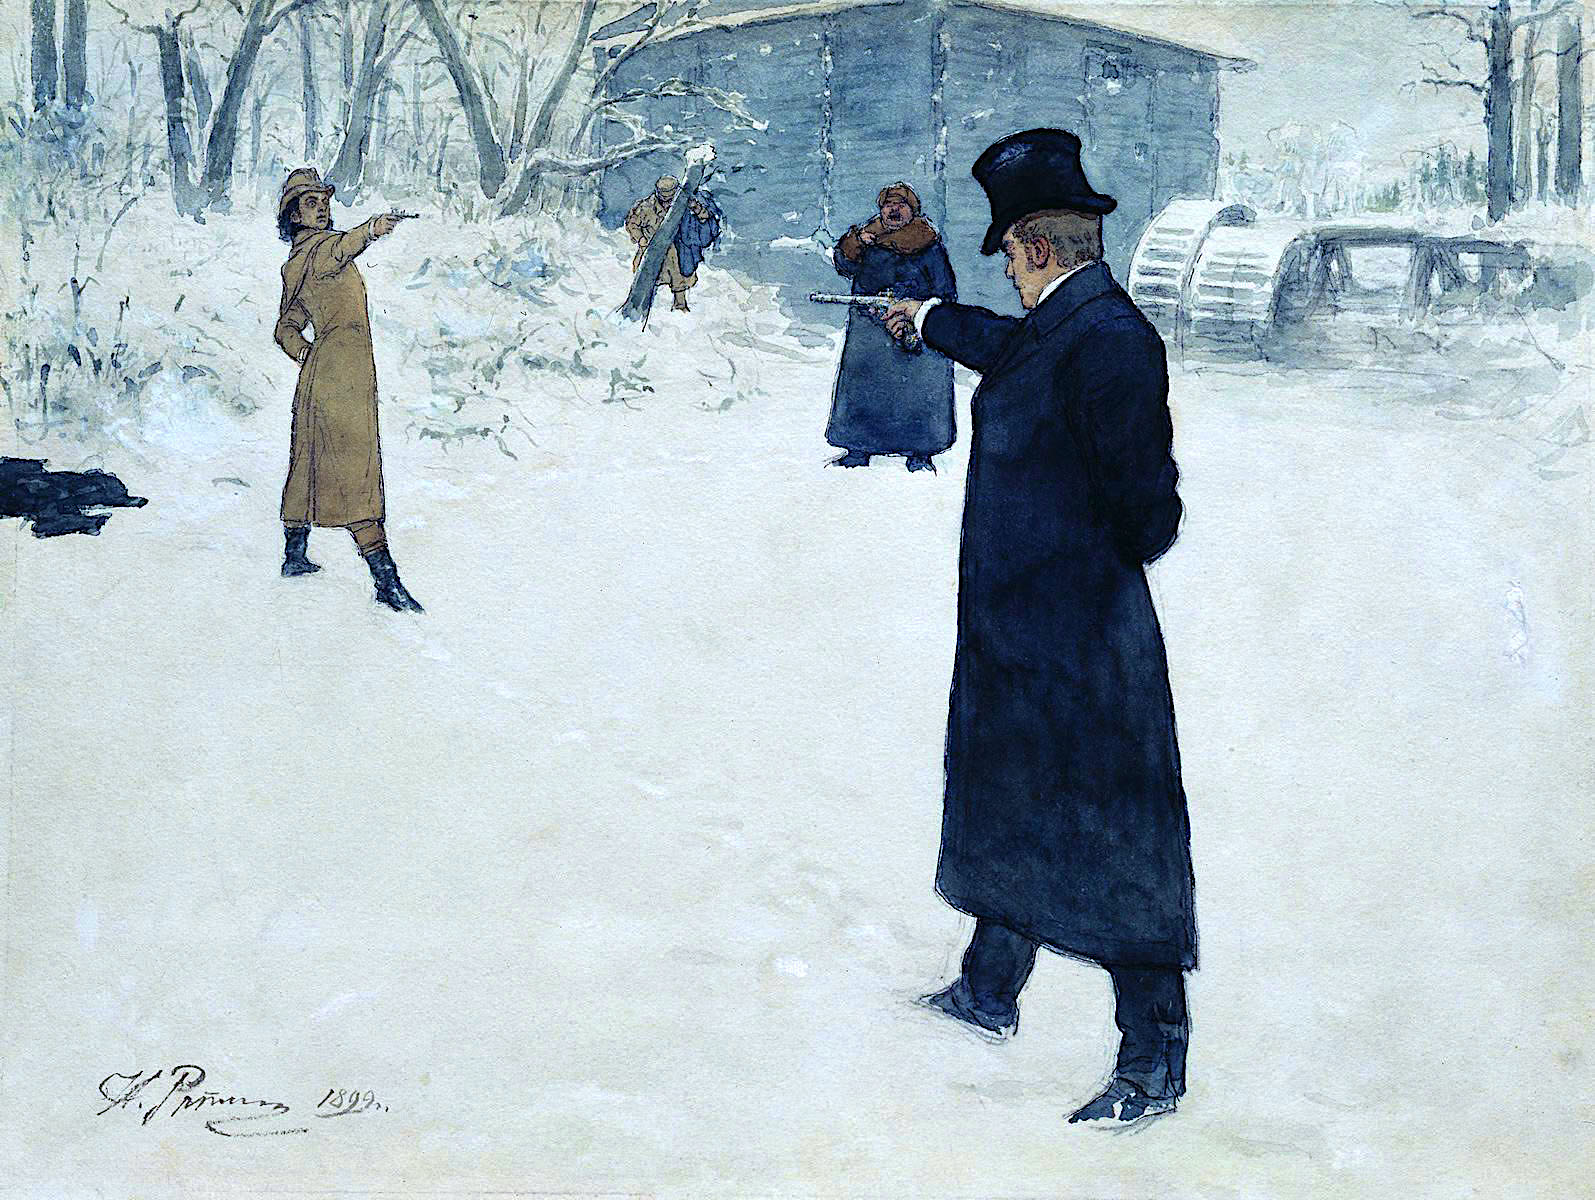
\includegraphics[width=0.8\textwidth]{Eugene}\\
            \vspace{1.5cm}
 
            % Author information
            {\large\spacedlowsmallcaps{By}\par}
            \vspace{0.5cm}
            {\Large\spacedallcaps{\@author}\par}
            \vspace{1cm}
            
            % Department and date
            {\large Department of Mathematics\par}
            \vspace{0.2cm}
            {\large Higher School of Economics\par}
            \vspace{0.5cm}
            {\large \@date\par}

            \vfill

            % Publisher logo at bottom
            
\includegraphics[width=0.2\textwidth]{Logo_HSE.png}
        \end{center}
    \end{titlepage}
    
    % Explanation page (new page after title page)
    \thispagestyle{empty}
    \vspace*{\fill}
    \begin{center}
        \begin{minipage}{0.8\textwidth}
            \centering
            \large\itshape
            Illustration from Alexander Pushkin's ``Eugene Onegin.''\\
            The poem has been object of the first stattistical study\\
	    involving Markov Chains. 
            \vspace{1cm}
        \end{minipage}
    \end{center}
    \vspace*{\fill}
    \clearpage
}
\makeatother


%
%% Title page customization
%\makeatletter
%\renewcommand{\maketitle}{%
%    \begin{titlepage}
%        \begin{center}
%            \vspace*{1.5cm}
%            
%            % University logo at top
%            
\includegraphics[width=0.3\textwidth]{logo-orizzontale-completo.jpg}\\
%            \vspace{1cm}
%
%            % Title with decorative rule
%            {\singlespacing\LARGE\spacedlowsmallcaps{\@title}\par}
%            \vspace{0.4cm}
%            \rule{0.5\textwidth}{0.4pt}\par
%            \vspace{1.5cm}
%
%            % Featured image with explanation
%            \begin{minipage}{0.9\textwidth}
%                \centering
%                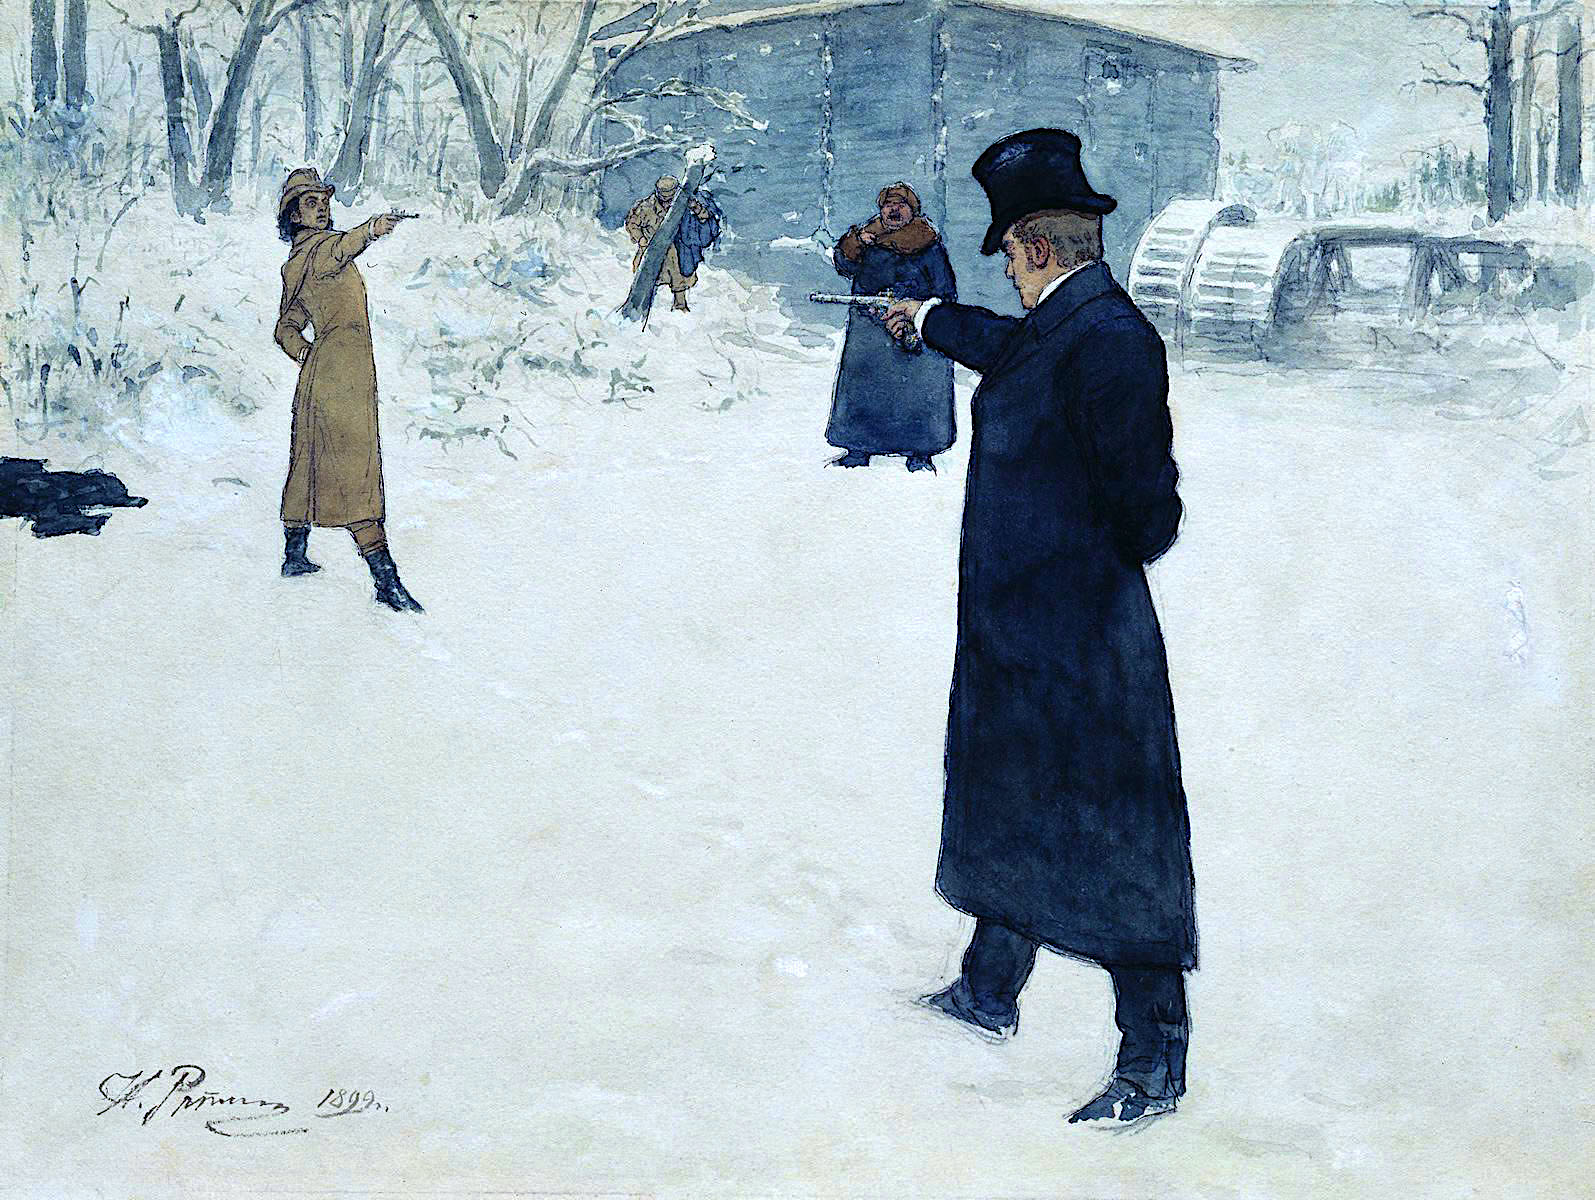
\includegraphics[width=\linewidth]{Eugene}\\
%                \vspace{0.5cm}
%                \begin{minipage}{0.8\linewidth}
%                    \small\itshape
%                    The duel scene from Alexander Pushkin's ``Eugene Onegin,'' 
%                \end{minipage}
%            \end{minipage}
%            \vspace{1.5cm}
% 
%            % Author information
%            {\large\spacedlowsmallcaps{By}\par}
%            \vspace{0.5cm}
%            {\Large\spacedallcaps{\@author}\par}
%            \vspace{1cm}
%            
%            % Department and date
%            {\large Department of Statistics\par}
%            \vspace{0.2cm}
%            {\large University of Data Science\par}
%            \vspace{0.5cm}
%            {\large \@date\par}
%
%            \vfill
%
%            % Publisher logo at bottom
%            
\includegraphics[width=0.2\textwidth]{logo-orizzontale-completo.jpg}
%        \end{center}
%    \end{titlepage}
%}
%\makeatother
%
%%%%%%%%%%%%%%%%%%%%%%%%%%%%%%%%%%%%%%%%%%%%%%%%%%%%%%%%%%%%%%%%%%%
%%%%%%%%%%%%%%%%%%%%%%%%%% EXAMPLE ENVIRONMENT %%%%%%%%%%%%%%%%%%%%
%%%%%%%%%%%%%%%%%%%%%%%%%%%%%%%%%%%%%%%%%%%%%%%%%%%%%%%%%%%%%%%%%%%


% ===== Add to preamble.tex =====
\usepackage{tcolorbox}
\tcbuselibrary{skins, breakable}

% Define example environment
\newcounter{example}[chapter]
\renewcommand{\theexample}{\thechapter.\arabic{example}}

\definecolor{examplecolor}{RGB}{13,85,160}  % Deep blue for header
\definecolor{examplebg}{RGB}{240,248,255}   % Light blue for background

\newenvironment{example}[1][]{%
  \refstepcounter{example}%
  \vspace{1em}%
  \begin{tcolorbox}[
    enhanced,
    breakable,
    title={\textbf{Example \theexample\if\relax\detokenize{#1}\relax\else: #1\fi}},
    coltitle=white,
    colbacktitle=examplecolor,
    colback=examplebg,
    colframe=examplecolor,
    fonttitle=\sffamily\bfseries,
    attach boxed title to top left={xshift=5mm, yshift=-2mm},
    boxed title style={size=small, colback=examplecolor},
    before skip=10pt,
    after skip=10pt,
    top=10pt,
    bottom=10pt
  ]
}{\end{tcolorbox}\vspace{0.5em}}
% ===== End addition =====



\usepackage{tikz}
\usetikzlibrary{decorations.pathreplacing}


\usepackage{amssymb}
\usepackage{amsmath}
%\usepackage{sidenotes}

\usepackage{amsthm}
\usepackage{mathtools}
\mathtoolsset{showonlyrefs}
\usepackage[notcite,notref]{showkeys}
\usepackage[backend = biber, style = numeric]{biblatex}
\usepackage{enumitem}
\usepackage[printsolution=true]{exercises}
\usepackage{exercise}


%\usepackage[
%  pdfpagemode={UseOutlines}, % show bookmarks panel when opening
%  bookmarks=true,            % create bookmarks
%  bookmarksopen=true,        % expand them by default
%  bookmarksopenlevel=1,      % depth to which bookmarks are open
%  bookmarksnumbered=true,    % number the bookmarks
%  hypertexnames=false,       % avoid duplicate anchors
%  colorlinks=true,           % colored instead of framed links
%  linkcolor=red,         % color for internal links
%  citecolor= green,         % citations
%  urlcolor=magenta,          % external links
%  filecolor=magenta,         % local files
%  pdfstartview={FitV},       % fit vertically on open
%  unicode=true,              % allow unicode in bookmarks
%  breaklinks=true            % allow line breaks in links
%]{hyperref}

% \usepackage{acronym}
% \usepackage{breqn}
% \usepackage[mathscr]{euscript}
% \usepackage[small]{caption}
% \usepackage{psfrag}

% \usepackage{mathrsfs}
% \usepackage{tikz}
% \usepackage{color}
% \usepackage{enumitem}
%\usepackage{enumerate}

\newcommand{\sidenote}[1]{%
        \refstepcounter{sidenote}\mbox{\textsuperscript{\alph{sidenote}}}%
        \marginpar{\footnotesize \mbox{\textsuperscript{\alph{sidenote}} }#1}%
}
\newcounter{sidenote}

\newcommand{\subscript}[2]{$#1 _ #2$}

%\renewcommand\theequation{\thesection.\arabic{equation}}
%\renewcommand\thefigure{\arabic{figure}}
%\renewcommand\thetable{\thesection.\arabic{table}}
%\bibliographystyle{plain} % We choose the "plain" reference style



\newcommand{\mc}[1]{{\mathcal #1}}
\newcommand{\mf}[1]{{\mathfrak #1}}
\newcommand{\mb}[1]{{\mathbf #1}}
\newcommand{\bb}[1]{{\mathbb #1}}

\newcommand{\bs}[1]{{\boldsymbol #1}}
\newcommand{\ms}[1]{{\mathscr #1}}


\newcommand{\mt}[1]{{\texttt #1}}

\newcommand{\<}{{\langle \!\! \langle}}
\renewcommand{\>}{{\rangle \!\! \rangle}}

\newcommand{\bel}[2]{\begin{equation} \label{#1} \begin{split} #2
 					\end{split} \end{equation}}


\newcommand{\mmu}{{\pmb \mu}}
\newcommand{\jj}{{\pmb j}}

%%%%%COMMENT
\usepackage{color}
\definecolor{light}{gray}{.90}
\newcommand{\commento}[1]{
	%%$\phantom .$ %higher inteline before comment
	\par\noindent
	\colorbox{light}{\begin{minipage}{120 mm}#1\end{minipage}}
	\par\noindent
}


\parindent0pt


\AddToHook{cmd/section/before}{\clearpage}


\addbibresource{Stat_biblio.bib}

\title{ An Introduction to Statistics using R}
\author{Alessandro Gubbiotti}


%%%%%%%%%%%%%%%%%%%%%%%%%%%%%%%%%%%%%%%%%%%%%%%%%%%%%%%%%%%%%%%%%%%%
%%%%%%%%%%%%%%%%%%%%%%%%%%%%%%%%%%%%%%%%%%%%%%%%%%%%%%%%%%%%%%%%%%%%
%%%%%%%%%%%%%%%%% DEEPSEEK TITLE PAGE WITH FIGURE %%%%%%%%%%%%%%%%%%
%%%%%%%%%%%%%%%%%%%%%%%%%%%%%%%%%%%%%%%%%%%%%%%%%%%%%%%%%%%%%%%%%%%%
%%%%%%%%%%%%%%%%%%%%%%%%%%%%%%%%%%%%%%%%%%%%%%%%%%%%%%%%%%%%%%%%%%%%
%%%
%%% The image 
%%%
% Add to your preamble.tex
\usepackage{tikz}
\usetikzlibrary{calc,patterns,decorations.pathmorphing}

% Central Limit Theorem visualization
\newcommand{\cltimage}{%
\begin{tikzpicture}[scale=0.7, every node/.style={font=\small}]
  % Colors
  \definecolor{dist1}{RGB}{200,50,50}
  \definecolor{dist2}{RGB}{50,150,50}
  \definecolor{dist3}{RGB}{50,100,200}
  \definecolor{normal}{RGB}{180,0,180}
  
  % Population distributions
  \begin{scope}[shift={(0,5)}]
    % Uniform distribution
    \draw[dist1, thick] (0,0) -- (2,0) -- (2,1) -- (0,1) -- cycle;
    \node[dist1] at (1,-0.5) {Uniform};
    
    % Skewed distribution
    \draw[dist2, thick, shift={(3,0)}] 
      plot[domain=0:2, samples=50] (\x, {0.5*exp(-0.5*\x)*\x});
    \node[dist2] at (4,-0.5) {Exponential};
    
    % Discrete distribution
    \draw[dist3, thick, shift={(6,0)}] 
      (0,0) -- (0.5,0) -- (0.5,1) -- (1.5,1) -- (1.5,0.5) -- (2,0.5) -- (2,0);
    \node[dist3] at (7,-0.5) {Discrete};
  \end{scope}
  
  % Arrow to sampling distribution
  \draw[->, thick] (3.5,3.8) -- (3.5,2.5) node[midway, right] {Sample Means};
  
  % Sampling distributions
  \begin{scope}[shift={(0,0)}]
    % n=5
    \draw[thick] (1,0) -- (1,0.5) -- (1.5,0.8) -- (2,1) -- (2.5,0.8) -- (3,0.5) -- (3,0);
    \node at (2,-0.5) {n=5};
    
    % n=15
    \draw[thick, shift={(3.5,0)}] 
      plot[domain=0:3, samples=50] (\x, {0.7*exp(-(\x-1.5)^2/0.4)});
    \node at (5,-0.5) {n=15};
    
    % n=30 (normal distribution)
    \draw[normal, very thick, shift={(6,0)}] 
      plot[domain=0:3, samples=100] (\x, {1.2*exp(-(\x-1.5)^2/0.2)});
    \node[normal] at (7.5,-0.5) {n=30};
    
    % Normal curve label
    \node[normal] at (7.5,2) {Normal Distribution};
    \draw[normal, ->] (7.5,1.8) -- (7.5,1.2);
  \end{scope}
  
  % Central Limit Theorem label
  \node[align=center, font=\bfseries] at (3.5,6) {
    \large Central Limit Theorem \\
    \footnotesize Sample means approach normal distribution \\ 
    \footnotesize as sample size increases
  };
  
  % Decorative elements
  \draw[decorate, decoration={snake, amplitude=0.5mm}, gray] (0.5,4.5) -- (6.5,4.5);
  \foreach \x in {1,2,...,7} {
    \draw[fill=black] (\x,4.5) circle (0.05);
  }
\end{tikzpicture}
}

% Replace the existing title page definition with this:
%%\makeatletter
%%\renewcommand{\maketitle}{%
%%    \begin{titlepage}
%%        \begin{center}
%%            % University logo
%%            
\includegraphics[width=0.25\textwidth]{logo-orizzontale-completo.jpg}\\
%%            \vspace{1cm}
%%            
%%            % Title - using \textls instead of \spacedlowsmallcaps
%%            {\singlespacing\LARGE\textls[100]{\textsc{\@title}}\par}
%%            \vspace{0.4cm}
%%            \rule{0.6\textwidth}{0.4pt}\par
%%            \vspace{1cm}
%%            
%%            % Central Limit Theorem graphic
%%            \cltimage
%%            \vspace{1cm}
%%            
%%            % Author information - using \textsc for small caps
%%            {\large\textsc{By}\par}
%%            \vspace{0.5cm}
%%            {\Large\textsc{\@author}\par}
%%            \vspace{1cm}
%%            
%%            % Department and date
%%            {\large Department of Statistics\par}
%%            \vspace{0.5cm}
%%            {\large \@date\par}
%%            
%%            \vfill
%%            % Publisher logo
%%            
\includegraphics[width=0.15\textwidth]{logo-orizzontale-completo.jpg}
%%        \end{center}
%%    \end{titlepage}
%%}
%%\makeatother
%
%
%%%%%% THE TITLE PAGE IT DOES NOT WORK SINCE IT IS NOT ABLE TO USE THE COMMANDS OF CLASSIC THESIS FOR THE TITLE PAGE 
%% Modify your maketitle command in preamble.tex
%\renewcommand{\maketitle}{%
%    \begin{titlepage}
%        \begin{center}
%            % University logo
%            
\includegraphics[width=0.25\textwidth]{logo-orizzontale-completo.jpg}\\
%            \vspace{1cm}
%            
%            % Title
%            {\singlespacing\LARGE\spacedlowsmallcaps{\@title}\par}
%            \vspace{0.4cm}
%            \rule{0.6\textwidth}{0.4pt}\par
%            \vspace{1cm}
%            
%            % Central Limit Theorem graphic
%            \cltimage % <--- Insert the graphic here
%            \vspace{1cm}
%            
%            % Author information
%            {\large\spacedlowsmallcaps{By}\par}
%            \vspace{0.5cm}
%            {\Large\spacedallcaps{\@author}\par}
%            \vspace{1cm}
%            
%            % Department and date
%            {\large Department of Statistics\par}
%            \vspace{0.5cm}
%            {\large \@date\par}
%            
%            \vfill
%            % Publisher logo
%            
\includegraphics[width=0.15\textwidth]{logo-orizzontale-completo.jpg}
%        \end{center}
%    \end{titlepage}
%}
%
